\chapter{Hybrid Evolutionary approach}
\label{chap:methodology}
%\minitoc



\section{Hybrid Genetic Algorithm}

A evolutionary algorithm is a technique bio-inspired in the evolution of some structures, it was proposed in first time by John Holland in the 60's, this algorithm seeks to evolve a population of individuals that represent solutions to the problem through genetic operators such as crossover, mutations and selection, the population generated in each iteration is evaluated and then the individuals that had a better fitness are chosen for the next generation with more probability.

A hybrid evolutionary algorithm or hybrid genetic algorithm are very popular techniques that offers practical advantages to deal with complex and hardly optimization problems. (Grosan, 2007) present a review of hybrid genetic architectures frecuently used.

``Evolutionary algorithm behavior is determined by the exploitation (improve solution - local search) and exploration (avoid local optimum extending the search space) relationship kept throughout the run''

hibridization is used for:
Improve the performance of the evolutionary algorithms
Improve quality of solutions obtained by evolutionary algorithm
Incorporate evolutionary algorithm as part of a large system

hybridization can be performed using prior knowledge, heuristics, local search, other techniques

local search is knowed as memetic algorithm

local search can be incorporated in the initial population or among the offsprings

\subsection{A basic genetic algorithm for vehicle routing problem with stochastic demands}

A example of a basic GA used to find solutions to VRPSD is showed in general form in figure \ref{fig:ga_basic}. First a initial population is selected, for each individual in the population assess fitness function, since individuals with better fitness function has more chance to reproduce then croossover operators are applied to selected individuals, also mutations can be performed in this stages, generating a offspring with new individuals. Probably, they will be added to new population whether have a fitness competitive respect to the population. So, a selection of individuals is applied to conform the new population, individuals with better fitness have more probability to get it. Until stopping criteriums are resolve, reproduction and selection is applied repeatedly over the population.

\begin{figure}[!htbp]
  \begin{center}
   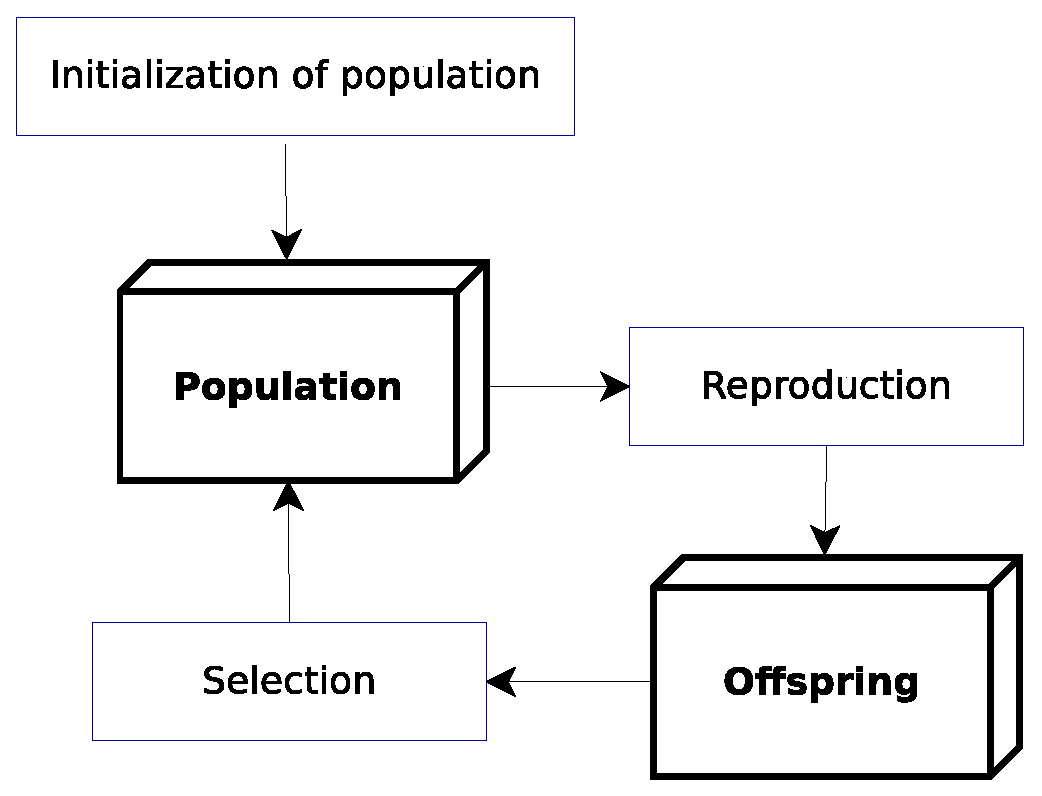
\includegraphics[width=0.6\textwidth]{Images/Chapter3/ga_basic.eps}
  \end{center}
    \caption{Basic genetic algorithm}\label{fig:ga_basic}
\end{figure}

Often hybridazation is included in inicialization and reproduction operators.

What is The fitness function? %answer

The crossover operator consist in selecting two different individuals $I_1$ and $I_2$ with probability dependently of their fitness value respectively, in contrast a random cut point $\gamma$ is selected uniformly $\gamma \in [1,n]$, then a new individual raise of concatenate the part $I_1$ sequence of 1 to the cut point with the part of sequence $I_2$ of cut point to $n$, at some times this process can be inverted, e.g. $I_1 = \{2, 3, 4, 5, 1\}$, $I_2= \{2, 3, 4, 1, 5\}$, then $I_1\times I_2 = \{2, 3, 4, 1, 5\}$. When a element in the crossover process can be generate a unfeasible sequence is corrected.

The mutation can happened with probability $\alpha = 0.2$ in the experiments presented in this document, this operator swaps two elements of an tour selected randomly.


A classic genetic algorithm does not yield competitive results, due to simple GA does not exploit problem knowing to produce high quality solutions. To be effective, we combine local search methods.


We represents individuals as a policy tour


Size of population:

Deprecated:
Size of population is $\lfloor \alpha \log n \rfloor$ where $\alpha$ is a tuneable parameter which should be fixed depending of computational resources 

Used:
Size of population is $\lfloor \max \{ n+\alpha(n\Delta_{E'}), n/4 \} \rfloor$ where $\alpha$ is a tuneable parameter which should be fixed depending of computational resources, it reward a offspring that improve the quality of the solutions regard to theirs parents increasing the population size, otherwise, when the quality of the solutions decrease the size of population is punished.


\subsection{Genetic operators}

\subsubsection{Crossover - EAX}

Edge assembly crossover

\subsubsection*{Mutation}

Swap

\subsubsection*{local search}

\subsubsection*{Performance of the genetic algorithm}

This section describes the algorithm performance for a specific problem instance with 10 customers and a factor $f'=1$, the customers' location and demand value (known when the vehicle arrive to the customer location) are showed in the figure \ref{fig:customer_n10_f1_s1}.


%\begin{figure}[!htbp]
%  \begin{center}
%    \includegraphics[width=0.9\textwidth]{Chapitre3/n10_f1_s1_customers}
%  \end{center}
%    \caption{Instance features: $n = 10$, $seed = 1$, $f' = 1$}\label{fig:customer_n10_f1_s1}
%\end{figure}

The genetic algorithm outcome for the instance problem described above is presented in the figure \ref{fig:tour_n10_f1_s1}, the red line describes the route, the segmented black line represents returns to the depot for replenishment, this tour was selected as the best solution found in 100 iterations of the GA.

%\begin{figure}[!htbp]
%  \begin{center}
%    \includegraphics[width=0.9\textwidth]{Chapitre3/n10_f1_s1_tour}
%  \end{center}
%      \caption{e.g best tour found by the GA: $n = 10$, $seed = 1$, $f' = 1$}\label{fig:tour_n10_f1_s1}
%\end{figure}

The figure \ref{fig:improve_n10_f1_s1} shows the improving of the objective function found, the chart shows the lesser total cost history, when a better value is found the line fall, therefore we can see the improving is given among the iteration 25 and 40, after this iterations the algorithm converges and it's not found a better solution.

%\begin{figure}[!htbp]
%  \begin{center}
%    \includegraphics[width=0.9\textwidth]{Chapitre3/n10_f1_s1_history}
%  \end{center}
%      \caption{e.g improvement solution: $n = 10$, $seed = 1$, $f' = 1$}\label{fig:improve_n10_f1_s1}
%\end{figure}

%\section{Memetic Algorithm}

%GA that use local search

%\section{Non-dominated Genetic Algorithm}

